\section{Diaframma} \label{sec:diaframma}
Il diaframma è un ghiera regolabile, composta da lamelle, che permette di controllare quanta luce colpisce il sensore. È posto all'interno dell'obiettivo.

Quando è completamente aperto le lamelle spariscono e la luce segue tutta la circonferenza della lente; man mano che viene chiuso la lamelle iniziano a formare un "cerchio" che fa da collo di bottiglia alla luce.

Il collo di bottiglia che forma il diaframma non è esattamente circolare, dipende da quante lamelle è composto il diaframma. Obiettivi più economici hanno il diaframma composto da 5 lamelle, quindi la luce passa sottoforma di pentagono; obiettivi di fascia più alta hanno più lamelle. Più lamelle ci sono più il diaframma si avvicina ad essere un cerchio.
Il concetto è lo stesso di quello visto con le lenti catadiottriche (vedi \nameref{subsec:lenticatadiottriche}), che fanno passare la luce a mo' di ciambella.

Come già visto il diaframma influenza l'esposizione di una foto, ma influenza altri due fattori:
\begin{itemize}
    \item[-] \textbf{\nameref{subsec:diaframmapdc}}
    \item[-] \textbf{\nameref{subsec:diaframmanitidezza}}
\end{itemize}

Chiudere il diaframma aiuta a risolvere anche diversi problemi: riduce la \textit{vignettatura}, riduce riflessi fastidiosi (quali \textit{flare}) e risolve problemi di \textit{distorsione} dell'immagine.
Vedi \nameref{sec:nomenclatura}.

\subsection{Profondità di campo} \label{subsec:diaframmapdc}
La \textbf{profondità di campo} è influenzata nel seguente modo: più è aperto il diaframma minore è la profondità di campo, e viceversa.

A seconda del tipo di fotografia che si vuole fare, e delle condizioni di luce, ci sono aperture che sono più consone, sia al tipo di scatto, sia ai gusti di chi scatta la foto.
Con un obiettivo da ritratti (es. 85mm) e molto aperto (es. $f/1.4$), se si vuole fotografare un volto da vicino tenere il diaframma completamente aperto può non piacere a molti: con un'apertura di 1.4 la profondità di campo è talmente ristretta cche non tutto il volto è a fuoco. Se infatti si mettono a fuoco gli occhi (nei ritratti si cerca solitamente di mettere a fuoco gli occhi) il naso potrebbe risultare fuori fuoco, e se il volto non è parallelo alla macchinetta allora si può mettere a fuoco solo un occhio.
Sono errori? Non necessariamente, possono essere scelte stilistiche, ma se si vuole mettere a fuoco tutto il volto le soluzioni sono due: allontanarsi dal soggetto oppure chiudere un po' il diaframma, così da aumentare la profondità di campo.

A seguire un esempio per vedere come una diversa apertura del diaframma influenzi la profondità di campo. Tutte le foto sono state scattate a circa 5cm dal muro, con una focale di 28mm.
Le foto verranno mostrate in due modi diversi:
\begin{itemize}
    \item[-] prima senza alcuna modifica
    \item[-] poi con un filtro che mette in evidenza la zona nitida di ogni immagine (ovvero la zona viola)
\end{itemize}

\begin{figure}[H] %!ht
    \centering
        \begin{subfigure}{0.45\linewidth}
            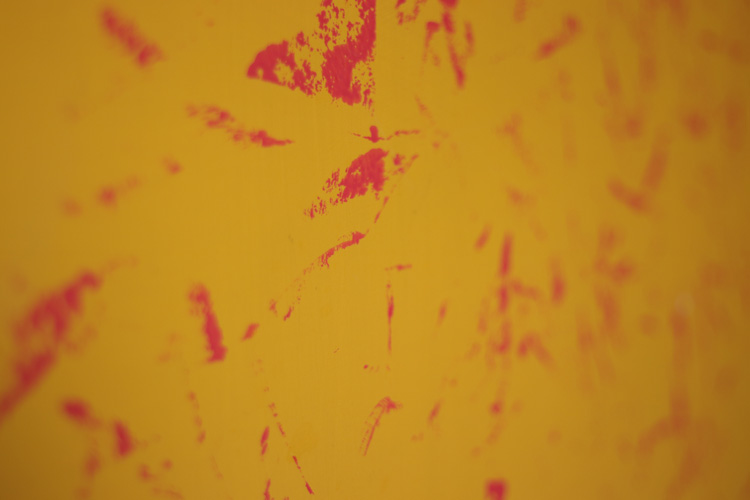
\includegraphics[width=\linewidth]{2.8.jpg}
            \caption{$f/2.8$}
        \end{subfigure}
    \hfil
        \begin{subfigure}{0.45\linewidth}
            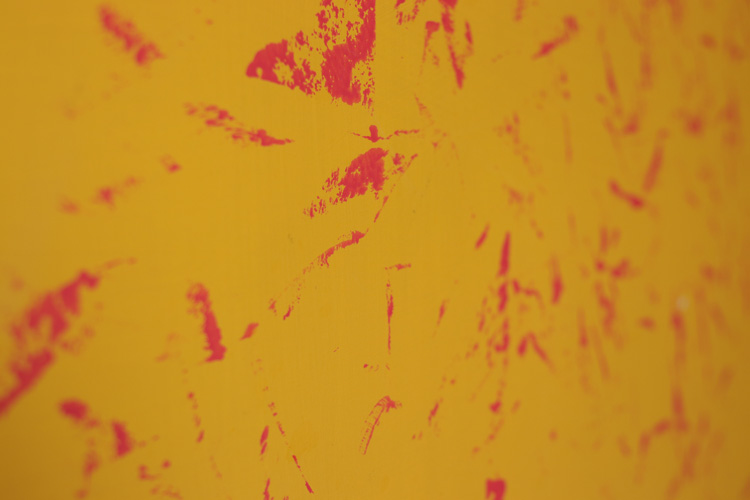
\includegraphics[width=\linewidth]{5.6.jpg}
            \caption{$f/5.6$}
        \end{subfigure}
    
        \begin{subfigure}{0.45\linewidth}
            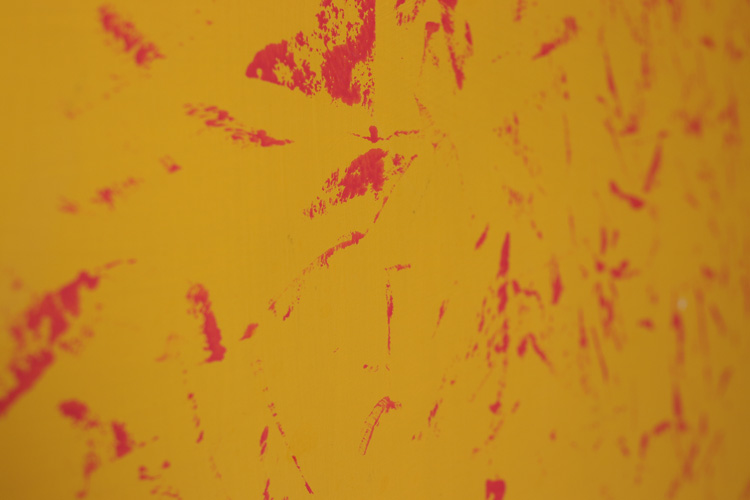
\includegraphics[width=\linewidth]{8.jpg}
            \caption{$f/8$}
        \end{subfigure}
    \hfil
        \begin{subfigure}{0.45\linewidth}
            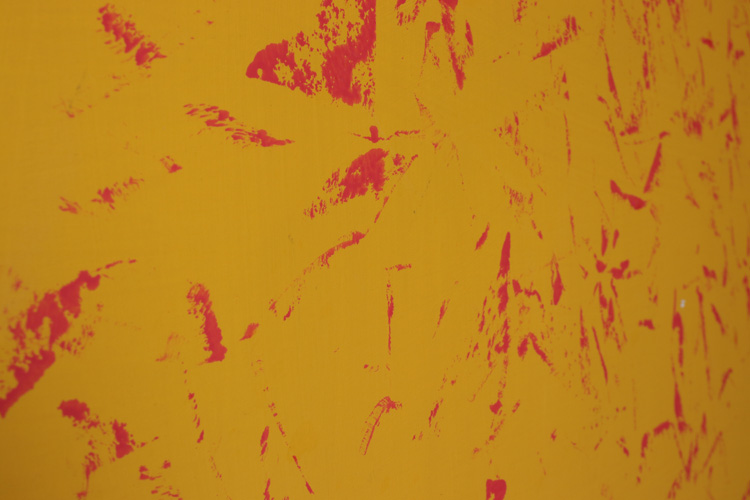
\includegraphics[width=\linewidth]{22.jpg}
            \caption{$f/22$}
        \end{subfigure}
    
    %\caption{2 x 3 grid of images}
    %\label{fig:diaframmadof}
\end{figure}

\begin{figure}[H]
    \centering
        \begin{subfigure}{0.45\linewidth}
            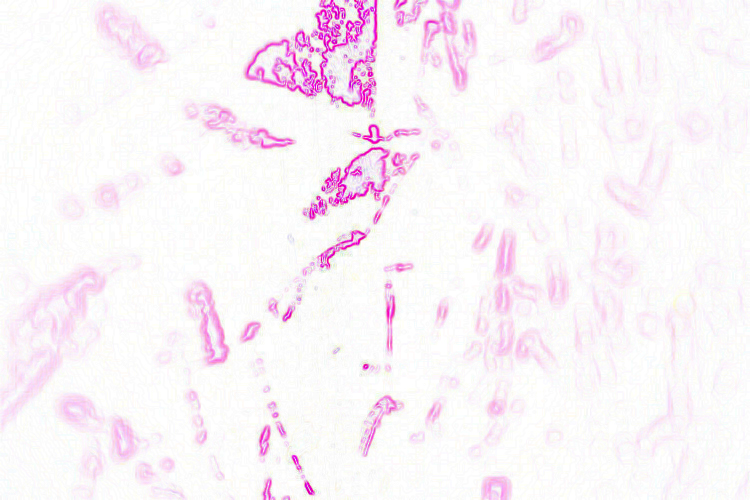
\includegraphics[width=\linewidth]{2.8_edges.jpg}
            \caption{$f/2.8$}
        \end{subfigure}
    \hfil
        \begin{subfigure}{0.45\linewidth}
            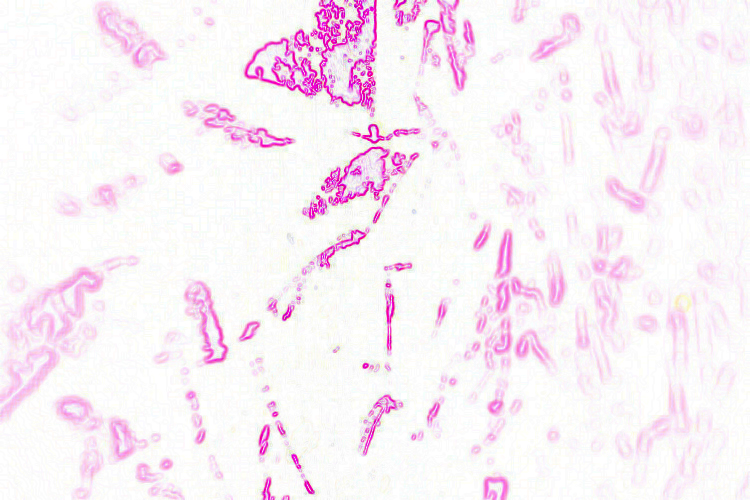
\includegraphics[width=\linewidth]{5.6_edges.jpg}
            \caption{$f/5.6$}
        \end{subfigure}
    
        \begin{subfigure}{0.45\linewidth}
            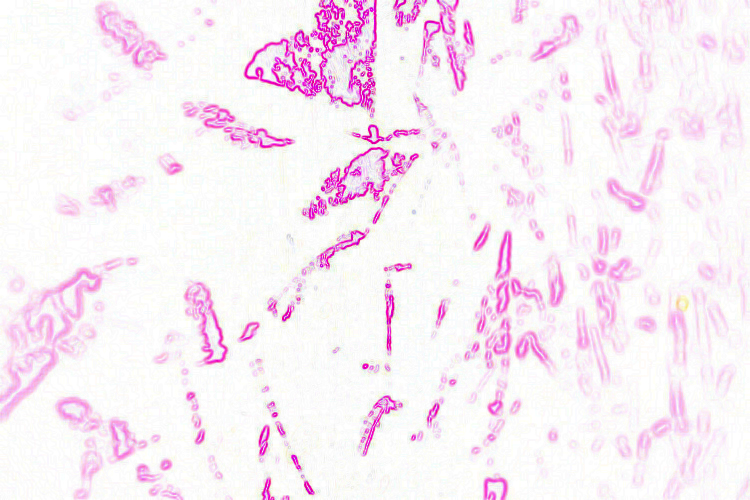
\includegraphics[width=\linewidth]{8_edges.jpg}
            \caption{$f/8$}
        \end{subfigure}
    \hfil
        \begin{subfigure}{0.45\linewidth}
            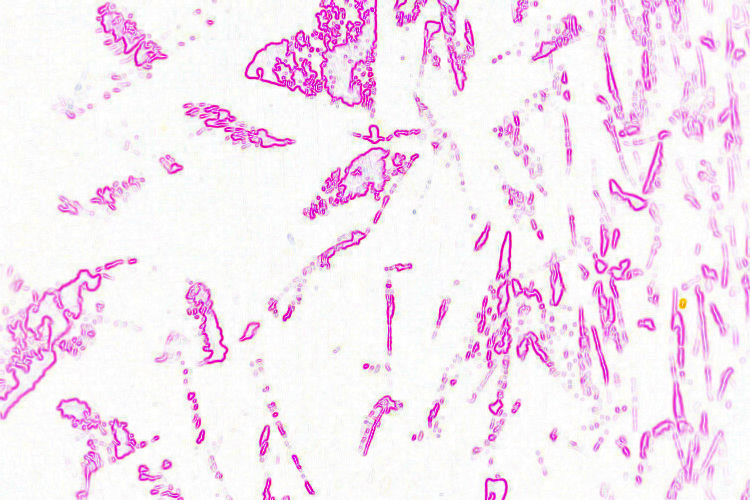
\includegraphics[width=\linewidth]{22_edges.jpg}
            \caption{$f/22$}
        \end{subfigure}
    
    \caption{In questo caso è evidente come, chiudendo il diaframma, la profondità di campo vada sempre aumentando}
    %\label{fig:diaframmadof}
\end{figure}


A seguire un altro esempio che mostra come chiudere il diaframma modifichi la forma delle luci fuori fuoco. Per le foto è stato usato un Canon \lens{50}{1.8}, che ha un diaframma a 5 lamelle.
\begin{figure}[H]
    \centering
        \begin{subfigure}{0.33\linewidth}
            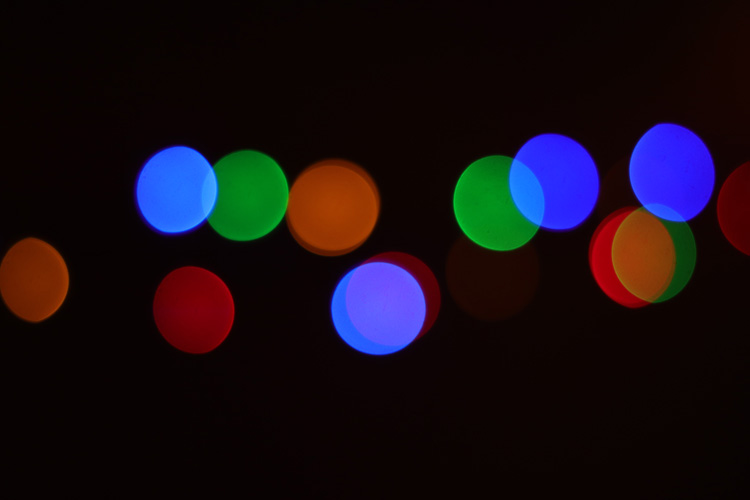
\includegraphics[width=\linewidth]{Luci_1.8.jpg}
            \caption{$f/1.8$}
        \end{subfigure}
    %\hfil
        \begin{subfigure}{0.33\linewidth}
            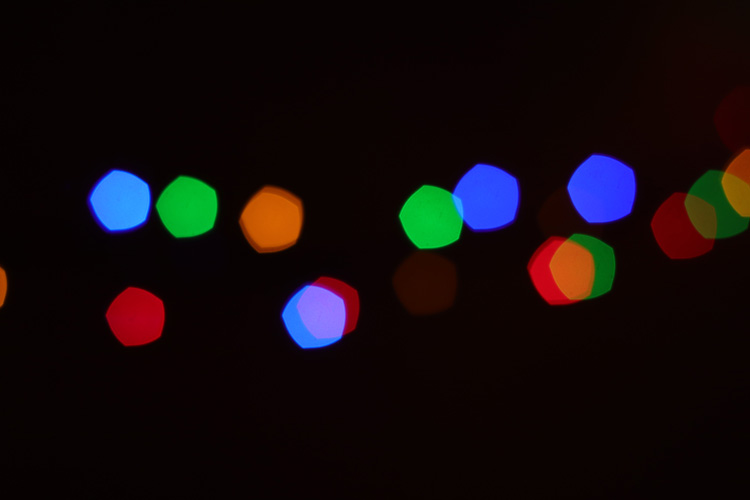
\includegraphics[width=\linewidth]{Luci_2.8.jpg}
            \caption{$f/2.8$}
        \end{subfigure}
    
        \begin{subfigure}{0.33\linewidth}
            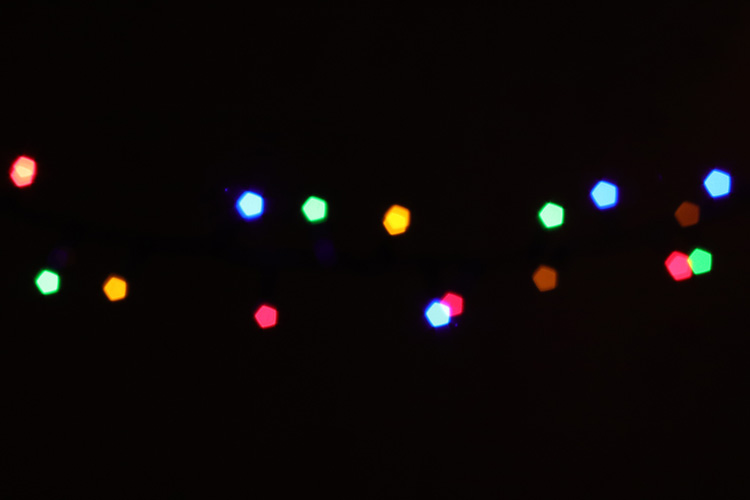
\includegraphics[width=\linewidth]{Luci_8.jpg}
            \caption{$f/8$}
        \end{subfigure}

    %\caption{2 x 3 grid of images}
    \label{fig:diaframmaluci}
\end{figure}

\subsection{Nitidezza} \label{subsec:diaframmanitidezza}
Con la \textbf{nitidezza} invece il discorso un po' cambia. Chiudendo il diaframma la nitidezza aumenta, ma solo fino ad un certo punto, superato il quale, se si continua a chiudere il diaframma, la nitidezza diminuisce nuovamente.

Ogni obiettivo ha un punto di massimo di nitidezza, quindi non si può dare una regola generale che funzioni sempre, si può però dare una regola empirica, che funziona spesso o che comunque è in grado di avvicinarsi alla realtà.
Molti obiettivi full frame e APS-C raggiungono il massimo della nitidezza intorno a $f/8$, più aperto o più chiuso di così perdono nitidezza.

Se invece parliamo di lenti per sensori più grandi la situazione è tutta diversamente, specialmente con le lenti per grande formato. A causa delle dimensioni usare grandi aperture fa calare drasticamente la nitidezza; le lenti grandi formato risentono così tanto di questo problema che il diaframma completamente aperto viene usato soltanto per avere più luce per comporre e mettere a fuoco l'inquadratura, si scatta poi con aperture come $f/22$ o più.


\subsection{Calcolare l'apertura} \label{subsec:calcolareapertura}
L'apertura massima di un obiettivo è espressa in \textit{f stop}, ed è un valore facilmente calcolabile.
\[ f = \dfrac{l}{d} \]

Dove:
\begin{itemize}
    \item[-] $f$ è l'apertura massima del diaframma
    \item[-] $l$ è la lunghezza focale 
    \item[-] $d$ è il diametro dell'obiettivo 
\end{itemize}
Per \textit{diametro} non si intende quello frontale dell'obiettivo, che noi vediamo da davanti, ma il diametro della lente dall'altra parte, quella sull'innesto, più vicina al sensore.


\subsection{T stop} \label{subsec:tstop}
Il diaframma, dato in $f$ stop, è un semplice valore calcolato; questo significa che due lenti con la stessa apertura non necessariamente avranno la stessa luminosità.
Detto in altre parole, se facciamo due foto, nelle stesse identiche condizioni di luce, stessi parametri, ma usiamo due obiettivi diversi, è possibile che le due foto siano esposte in modo diverso.

Il T stop (T per \textit{Transmission}) invece non ha questo problema, indica infatti la quantità di luce che la lente fa arrivare all'obiettivo.
Quindi se si usano due obiettivi con lo stesso T stop abbiamo la garanzia che la luminosità delle foto sia la stessa.

Lenti misurate in T stop sono solitamente pensate per fare video, non foto; hanno infatti, molto spesso, una serie di caratteristiche desiderabili per il video, spesso poco o per niente sfruttabili quando si scattano foto.

Queste caratteristiche sono:
\begin{itemize}
    \item[-] sono lenti completamente manuali (i.e. messa a fuoco, focale e diaframma si controllano solo a mano)
    \item[-] le ghiere di messa a fuoco e diaframma hanno dei denti molto grandi, che permettono di agganciare il follow focus (uno strumento che aiuta a ruotare le ghiere con più precisione)
    \item[-] la ghiera del diaframma non ruota a scatti, ma è continua
    \item[-] \textit{focus breathing} quasi del tutto assente
    \item[-] se sono lenti zoom spesso sono \textit{parafocali}
\end{itemize}

Cos'è il \textbf{focus breathing}?
Quando mettiamo a fuoco, l'obiettivo, anche se in maniera molto contenuta, va un po' avanti e indietro; di fatto è come se stessimo zoommando in maniera quasi impercettibile.
Se dobbiamo scattare una foto questo non è un problema, ma in video questo sfasamento è visibile e solitamente non molto gradito.

Cos'è una lente \textbf{parafocale}?
Quando andiamo a cambiare lo zoom di una lente (quindi parliamo di lenti zoom, non fisse) cambia anche la messa a fuoco.
Esempio: zoommo al massimo su un soggetto e lo messo a fuoco, se poi torno allo zoom minimo (quindi il più grandangolare possibile) la messa a fuoco è cambiata e il soggetto non è più a fuoco.
Questo ragionamento vale in entrambi i versi, ovviamente.

Le lenti parafocali non hanno questo problema: la messa a fuoco è costante, indipendentemente dallo zoom.

%\begin{figure*}[h]
%    \centering
%    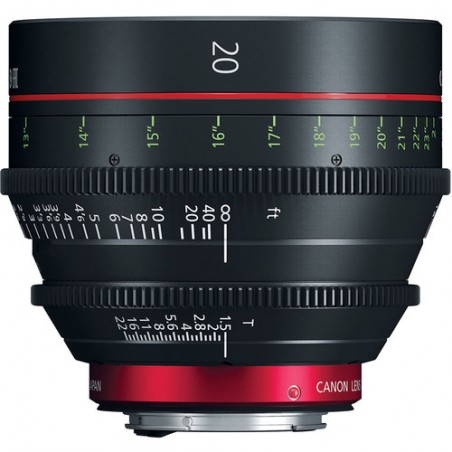
\includegraphics[width=0.42\textwidth]{canon_cine.jpg}
%    \label{fig:canon_cine}
%    \caption{Obiettivo Canon CN-E 20mm T 1.5}
%\end{figure*}